\documentclass[12pt]{article}
\usepackage{tikz}
\usepackage{graphicx}
\usepackage{amssymb}
\usepackage{amsmath}
\usepackage{mathtools}
\usepackage{amsthm}
\usetikzlibrary{arrows,automata,positioning}
\usepackage{enumitem}
\usepackage{todonotes}
\usepackage{fancyhdr}
\usepackage{wrapfig}
\usepackage{caption}
\captionsetup[table]{name=Tabelle}
\usepackage[ngerman]{babel}
\usepackage[utf8x]{inputenc}

\usepackage{geometry}
\geometry{
 a4paper,
 total={170mm,257mm},
 left=25mm,
 top=35mm,
 bottom=25mm,
 right=25mm
}
\newcommand{\rom}[1]{\uppercase\expandafter{\romannumeral #1\relax}}
\newcommand{\padTable}[1]{$\quad$ #1 $\quad$}
\newcommand{\ankerAuf}{⊣} % nur mit XeLaTeX, da Unicode!
\newcommand{\ankerZu}{⊢}
\pagestyle{fancy}
%\DeclareUnicodeCharacter{}{\ankerZu}
\fancyhf{}
\rhead{Klausur WiSe 2022}
\lhead{Mathematik \rom{3} $-$ Numerik}
\cfoot{Seite \thepage}
\lfoot{}


\usepackage{xcolor}
\usepackage{environ}
\usepackage[most]{tcolorbox}
\tcbset{on line,
        boxsep=4pt, left=0pt,right=0pt,top=0pt,bottom=0pt,
        colframe=white,colback=lightgray,
        highlight math style={enhanced}
        }
\newcommand{\kommentarMacro}[1]{\textcolor{lightgray}{(\texttt{#1})}}
\newcommand{\solutionMacro}[1]{\,\\\texttt{#1}\,\\}
\NewEnviron{solution}{\textcolor{blue}{\solutionMacro{\BODY}}}

\renewcommand{\footrulewidth}{1pt}
\title{Mathematik \rom{3} \\ Numerik \\ Lutz Gröll $-$ Klausur WiSe 2022}
\author{TINF21B1 \\ Lutz Gröll, Connaisseur der imaginären Schwarzwälder Kirschtorte}

\newsavebox\MBox
\newcommand\Cline[2][red]{{\sbox\MBox{$#2$}%
  \rlap{\usebox\MBox}\color{#1}\rule[-1.2\dp\MBox]{\wd\MBox}{0.5pt}}}


\begin{document}
\maketitle

\begin{center}
    \large
    \vspace*{7cm}
    Maximale Punktzahl: 69 Punkte\\
    \vspace*{1cm}
    Bearbeitungszeit: 90 Minuten\\
    \vspace*{1cm}
    Hilfsmittel: Taschenrechner + Formelblatt (für LA und Analysis, siehe Ordner)\\
    \vspace*{1cm}
    Datum: 06.12.2022\\
    \vspace*{1cm}
    \small \LaTeX-Dokument sowie teilweise Lösungen von 2021 übernommen \\Format der folgenden Seiten ist dem der Klausur sehr ähnlich.\\
\end{center}
\pagebreak



\section*{Aufgabe 1:}
\begin{enumerate}
    \item Notieren Sie die wichtigsten Schritte für das Erstellen eines numerischen Programms. \kommentarMacro{2022, 2021, 2019, 2018, 2016}
          \begin{solution}
              \begin{enumerate}[label=$(\roman*)$]
                  \item Geeigneten Algorithmus wählen
                  \item Ein- und Ausgabevariablen festlegen
                  \item Kommentare schreiben (Funktion des Programms, \\Spezifikation der Schnittstelle und Quelle)
                  \item Interne Variablen festlegen
                  \item Eigentliches Programm
                  \item Numerisches Testen
                  \item Optional: Optimieren
                  \item Numerische Bugs suchen und beseitigen
                  \item Andere Aspekte: Echtzeitanforderungen, Sicherheit
              \end{enumerate}
          \end{solution}
    \item Notieren Sie ein zweidimensionales Nullstellenproblem mit exakt 4 Lösungen (Formel und Skizze) \kommentarMacro{neu 2022, kein Originaltext}
          \begin{solution}
              $f(x,y)=\begin{bmatrix}
                      x^2 + y^2 - 1 \\ x^2 + 2 \cdot y^2 - 1.5
                  \end{bmatrix}$ \hspace{1.5cm}\raisebox{-.5\height}{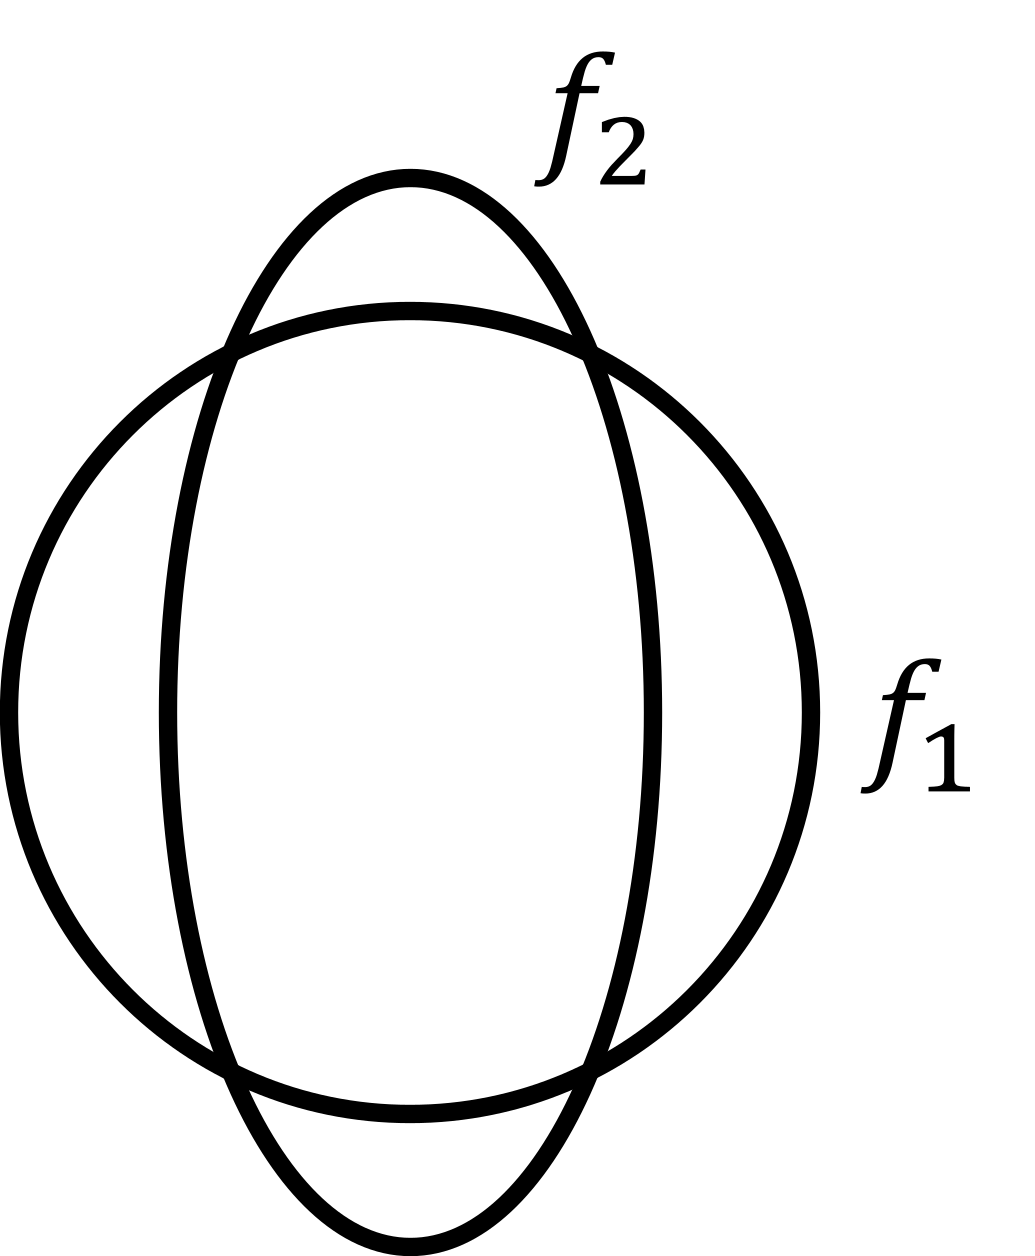
\includegraphics[width=0.125\textwidth]{4Loesungen.pdf}}
              \vspace{0.5cm}

              Hier wird effektiv nach dem Schnittpunkt eines Kreises mit \\ einer Ellipse gefragt.

              \rule{\textwidth}{0.4pt}

              Sollten nur 2 Lösungen verlangt sein, so reicht es aus \\ 2 verschobene Kreise zu nutzen:  $f(x,y)=\begin{bmatrix}
                      x^2 + y^2 - 1 \\ \left(x-1\right)^2 + y^2 - 1
                  \end{bmatrix}$.

              Ist nach unendlich vielen Lösungen gefragt, reicht das Vorkommen \\ der Faktorisierung einer Variable in beiden Formeln:
              $$f(x,y)=\begin{bmatrix}
                      \left(x^2-4\right)\cdot \left(y + 2\right) \\ \left(x+2\right)\cdot \left(y -2\right)
                  \end{bmatrix}=\begin{bmatrix}
                      \left(x-2\right)\cdot \left(x+2\right)\cdot \left(y+2\right) \\ \left(x+2\right)\cdot \left(y -2\right)
                  \end{bmatrix}$$

              Somit $x=-2$ und $y=$ beliebig. Natürlich lässt sich auch 2 mal der \\ gleiche Term angeben, jedoch ist Herr Gröll damit sicherlich nicht \\ begeistert.
          \end{solution}
    \item Nennen Sie ein ill-posed Problem für eine eindimensionale numerische Integration. \kommentarMacro{neu 2022, kein Originaltext}
          \begin{solution}
              $$\int\limits_{-1}^{1} \frac{1}{x}\hspace{0.1cm} dx$$
          \end{solution}
\end{enumerate}
\pagebreak

\newcommand{\spaltensummennorm}[1]{||#1||_{1}}
\newcommand{\zeilensummennorm}[1]{||#1||_{\infty}}
\newcommand{\realVector}[2]{#1\in \mathbb{R}^{#2}}
\newcommand{\realMatrix}[3]{#1\in \mathbb{R}^{#2\times #3}}
\newcommand{\indentTab}{\hphantom{~~~~}}

\section*{Aufgabe 2:}
\begin{enumerate}
    \item Geben Sie eine $2\times2$ Matrix an, welche verschiedene Konditionszahlen in der Spaltensummennorm und in der Zeilensummennorm hat. \kommentarMacro{neu 2022, kein Originaltext}

          \begin{solution}
              Ill-posed Problem. Die Konditionszahlen sind immer gleich. Da hat sich Herr Gröll bestimmt sehr amüsiert :)

              \rule{\textwidth}{0.4pt}
              \vspace{0.25cm}

              $A=\begin{bmatrix}
                      \text{a} & \text{b} \\ \text{c} & \text{d}
                  \end{bmatrix} \qquad A^{-1}=\frac{1}{det(A)}\begin{bmatrix}
                      \text{d} & -\text{b} \\ -\text{c} & \text{a}
                  \end{bmatrix}=\frac{1}{\text{a}\cdot\text{d}-\text{b}\cdot\text{c}}\begin{bmatrix}
                      \text{d} & -\text{b} \\ -\text{c} & \text{a}
                  \end{bmatrix}$

              \begin{align*}
                  \kappa_{1}(A) & = \spaltensummennorm{A} \cdot \spaltensummennorm{A^{-1}}                                                                                                                                                                                                                                                                                       \\
                                & = \max\left\{|a|+|c|,|b|+|d|\right\} \cdot \max\left\{\frac{|d|+|-c|}{|det(A)|},\frac{|-b|+|a|}{|det(A)|}\right\}                                                                                                                                                                                                                              \\
                                & = \max\left\{\Cline[green]{\frac{\left(|a|+|c|\right) \cdot \left(|c|+|d|\right)}{|det(A)|}},\Cline[red]{\frac{\left(|a|+|c|\right) \cdot \left(|a|+|b|\right)}{|det(A)|}},\Cline[lime]{\frac{\left(|b|+|d|\right)\cdot\left(|c|+|d|\right)}{|det(A)|}},\Cline[violet]{\frac{\left(|b|+|d|\right)\cdot\left(|a|+|b|\right)}{|det(A)|}}\right\}
              \end{align*}

              \begin{align*}
                  \kappa_{\infty}(A) & = \zeilensummennorm{A} \cdot \zeilensummennorm{A^{-1}}                                                                                                                                                                                                                                                                                         \\
                                     & = \max\left\{|a|+|b|,|c|+|d|\right\} \cdot \max\left\{\frac{|d|+|-b|}{|det(A)|},\frac{|-c|+|a|}{|det(A)|}\right\}                                                                                                                                                                                                                              \\
                                     & = \max\left\{\Cline[violet]{\frac{\left(|a|+|b|\right) \cdot \left(|b|+|d|\right)}{|det(A)|}},\Cline[red]{\frac{\left(|a|+|b|\right) \cdot \left(|a|+|c|\right)}{|det(A)|}},\Cline[lime]{\frac{\left(|c|+|d|\right)\cdot\left(|b|+|d|\right)}{|det(A)|}},\Cline[green]{\frac{\left(|c|+|d|\right)\cdot\left(|a|+|c|\right)}{|det(A)|}}\right\}
              \end{align*}

              Durch die Beträge lassen sich die Multiplikationen der $\max -$Funktionen \\ kombinieren. Wie zu erkennen ist, handelt es sich bei beiden Normen um das Gleiche.
          \end{solution}
    \item Formulieren Sie die Berechnung von $x = B^{-1}Cd$ in eine numerisch effiziente Form um. \kommentarMacro{2022, 2021}
          \begin{solution}
              $$Bx = Cd$$
          \end{solution}
    \item Zeigen Sie an einem Beispiel, dass die Addition numerisch nicht assoziativ ist. \\ \kommentarMacro{2022, 2021, 2012}
          \newcommand{\numPlus}{\,\widetilde{+}\,}
          \begin{solution}
              \begin{align*}
                  (10^{-20} \numPlus 1) \numPlus (-1) & \neq 10^{-20} \numPlus (1 \numPlus (-1)) \\
                  \iff \qquad \qquad \qquad \qquad 0  & \neq 10^{-20}
              \end{align*}
          \end{solution}

    \item Was verstehen Sie unter Overfitting? \kommentarMacro{neu 2022, kein Originaltext}

          \begin{solution}
              Das mathematische Modell hat zu viele Parameter, wodurch sich \\ die Approximation zu genau an die gegebenen Daten anpasst und \\ somit für zukünftige Daten unmbrauchbar wird.
              \begin{figure}[!ht]
                  \includegraphics[width=0.25\textwidth]{overfitting.png}
                  \centering
                  \vspace{-1cm}
              \end{figure}
          \end{solution}

    \item Was ist Spaltenskalierung? (Formel und Zweck/Anwendung) \\ \kommentarMacro{neu 2022, kein Originaltext}

          \begin{solution}
              $AD\underbrace{D^{-1}x}_{y}=b \implies \left(AD\right)y=b \quad\text{und}\quad x=Dy$

              Zweck ist die numerische Verbesserung beim Lösen \\ linearer Gleichungssysteme
          \end{solution}

    \item Sie haben ein schlecht konditioniertes Ausgleichsproblem aus dem ein Signal entstehen soll. Sie wollen dabei die 2. Ableitung bestrafen. Notieren Sie die Least-Square Formel, sowie die Matrix zur Bestrafung der 2. Ableitung. \\ \kommentarMacro{neu 2022, kein Originaltext}

          \begin{solution}
              $||Ax - b||_2^2 + \mu \cdot ||Lx||_2^2 \rightarrow Min$

              \vspace{0.35cm}

              $L=\begin{bmatrix}
                      2      & -1    & 0  & 0     & \dots  & 0      \\
                      -1     & 2     & -1 & 0     &        & \vdots \\
                      0      & -1    & 2  & -1    &        &        \\
                      0      & 0     & -1 & 2     &        & \vdots \\
                      \vdots &       &    &       & \ddots & -1     \\
                      0      & \dots &    & \dots & -1     & 2      \\
                  \end{bmatrix}$
              \vspace{1cm}

              $L$ ist eine Differenzenmatrix und enthält wie zu sehen die Gewichte der numerischen 2. Ableitung.
          \end{solution}
          \pagebreak
    \item Warum kann es beim Lösen der Differentialgleichung $\dot{x_1} = x_2 - k \sqrt{x_1}$ mit \mbox{$x\geq 0$} sinnvoll sein, eine Modifikation des Vektorfelds vorzunehmen? Welche Lösung schlagen Sie vor? \kommentarMacro{2022, 2021, 2020, 2019, 2018}

          \begin{solution}
              Durch numerische Fehler kann es passieren, dass $x_1 < 0$, sodass der Radikant negativ wird.\\
              Lösung: $\dot{x_1} = x_2 - k\sqrt{max\{x_1, 0\}}$

              - Verifiziert durch Herr Gröll.
          \end{solution}
    \item Wodurch sind Testmatrizen für numerische Leistungstests gekennzeichnet? \\ \kommentarMacro{2022, 2021, 2018, 2016}
          \vspace{-0.5cm}
          \begin{solution}
              \begin{enumerate}[label=$(\roman*)$]
                  \item In der Ordnung skalierbar \\ (zum Beispiel zum Testen des Speicherverbrauchs)
                  \item Lösung bekannt
                  \item Testen numerische Grenzfälle aus (Singularitäten, nahezu singulär etc.)
                  \item In der Kondition veränderlich
                  \item Stehen in Büchern!
              \end{enumerate}
          \end{solution}

\end{enumerate}
\pagebreak

\section*{Aufgabe 3:}
\begin{enumerate}
    \item Nennen Sie eine praktische Anwendung, für die eine Interpolation nach Lagrange in Frage kommt. \kommentarMacro{2022, 2021}

          \begin{solution}
              Bei Hashtabellen zum Berechnen eines Zwischenwertes (falls die\\ eigentliche Funktion zu aufwendig ist oder eine Approximation reicht).
          \end{solution}

    \item Notieren Sie für $y = \frac{ax + b}{x^2 + cx + d}$ einen linearen LS-Ansatz. \kommentarMacro{2022, 2021}

          \begin{solution}
              Ausmultiplizieren gibt $yx^2 + cyx + yd - ax - b = 0$. Daraus dann den LS-Ansatz:\\

              $Ax = 0_n,\qquad A = \begin{bmatrix}
                      y_1x_1^2 & y_1x_1 & y_1    & -x_1   & -1     \\
                      \vdots   & \vdots & \vdots & \vdots & \vdots \\
                      y_nx_n^2 & y_nx_n & y_n    & -x_n   & -1
                  \end{bmatrix}, \qquad x = \begin{bmatrix}
                      1 \\c\\d\\a\\b
                  \end{bmatrix}$.
          \end{solution}

    \item Wie viele Stützwerte benötigen Sie mindestens, um die Parameter aus Teilaufgabe 2 eindeutig bestimmen zu können? \kommentarMacro{2022, 2021}

          \begin{solution}
              4 Stützwerte
          \end{solution}

    \item In welchem Konflikt stehen Ingenieure, die online eine Ableitung berechnen müssen? \kommentarMacro{2022, 2021, 2018}

          \begin{solution}
              Sie kennen die zukünftigen Werte nicht und können um den neusten Wert deshalb niemals symmetrisch differenzieren.
          \end{solution}

    \item Was halten Sie von $f_k'' = -\frac{1}{12}f_{k-3}+ \frac{1}{3}f_{k-2} + \frac{1}{2}f_{k-1} - \frac{5}{3}f_k + f_{k+1}$? \\ \kommentarMacro{2022, 2021, 2018}

          \begin{solution}
              Gar nichts. Die Summe der Gewichte müssen beim Ableiten 0 sein (wegen $f(x) = c, c\in \mathbb{R}$. Außerdem muss man noch durch $h^2$ für die zweite Ableitung teilen.
          \end{solution}
          \pagebreak

    \item Erstellen Sie für die Formel $x^3\left(x-1\right)=1$ zwei verschiedene Fixpunktiterationen. \kommentarMacro{neu 2022, kein Originaltext}
          \begin{solution}
              \begin{align*}
                  x^3     & = \frac{1}{x-1}                                       & x-1     & =\frac{1}{x^3}                                \\
                  x_{x+1} & =\underbrace{\sqrt[3]{\frac{1}{x_k-1}}}_{\Phi_1(x_k)} & x_{k+1} & =\underbrace{\frac{1}{x_k^3}+1}_{\Phi_2(x_k)}
              \end{align*}
          \end{solution}
    \item Warum werden Eigenwerte von Matrizen numerisch nicht wie in der Algebra üblich über die charakteristische Gleichug bestimmt? Was macht man stattdessen? \\ \kommentarMacro{2022, 2021}

          \begin{solution}
              Da Polynome numerisch unvorteilhaft sind (Überläufe, aufwendige\\Berechnung und aufwendige Nullstellensuche). Bei $100\times 100$ Matrix ein\\Polynom 100. Grades. Stattdessen reelle QZ-Zerlegung \\(durch Gram-Schmidt-Orthogonalisierung).
          \end{solution}

    \item Skizzieren Sie eine instabile Fixpunktiteration graphisch. \\ \kommentarMacro{neu 2022, ähnlich zu 2019}
          \begin{solution}
              \begin{figure}[!ht]
                  \includegraphics[width=0.65\textwidth]{Fixpunktiteration.png}
                  \centering
              \end{figure}
          \end{solution}
\end{enumerate}
\pagebreak

\section*{Aufgabe 4:}
\begin{enumerate}
    \item Gegeben seien $\realMatrix{A}{30}{5}, \realMatrix{B}{5}{100}, \realVector{C}{100}$. Berechnen Sie die Flops für $A(BC)$. \\ \kommentarMacro{2022, sehr ähnlich zu 2021}

          \begin{solution}
              $D = BC, \realVector{D}{10},\qquad Flop(A(BC)) = \underbrace{Flop(AD)}_{30\cdot 1\cdot (2\cdot 5 - 1) = 270} + \underbrace{Flop(BC)}_{5\cdot 1\cdot (2\cdot 100 - 1) = 995} = 1265$
          \end{solution}

    \item Sie benutzen einen Microcontroller, der nur die 4 Grundrechenarten beherrscht. Damit müssen Sie öfters Polynome der Form $y=a_3x^3+a_2x^2+a_1x+a_0$ berechnen. Wie viele Flops werden bei einer einfachen Berechnung benötigt? Wie viele hingegen, wenn das Horner-Schema zur Berechnung verwendet wird? \\ \kommentarMacro{neu 2022, kein Originaltext}

          \begin{solution}
              Horner Schema: $y=\left(\left(\left(a_3\right)\cdot x + a_2\right)\cdot x + a_1\right)\cdot x + a_0$ \\
              \begin{align*}
                  Flop_{normal} & = 7\text{, wenn } x^3 \text{ durch } x^2 \cdot x \text{ berechnet wird, sonst } 9 \\
                  Flop_{horner} & = 6
              \end{align*}
          \end{solution}
    \item Welche Vorraussetzung muss für eine Parallelisierung eines Programms vorliegen? Nennen Sie ein Beispiel, wo Prallelisierung auf 8 Rechnerkernen leicht anwendbar ist und viel bringt. \kommentarMacro{2022, 2021, 2019, 2018}

          \begin{solution}
              Unabhängige Teilaufgaben. \\
              Beispiel: Matrixmultiplikation mit Matrizen $\realMatrix{A}{8}{8}, \realMatrix{B}{8}{8}, \\ A\cdot B = C$
          \end{solution}

    \item Schreiben Sie in Pseudocode einen Test, um numerische Bugs bei der Auswertung von $tan\,x$ zu verhindern. \kommentarMacro{2022, 2021, 2020, 2018, 2016}

          \begin{solution}
              double ownTangent(double x)\\
              \indentTab x' := (x  - $\frac{\pi}{2}$) mod $\pi$\\
              \indentTab if ($abs(x') \leq eps$) throw error\\
              \indentTab else return tan(x)\\
          \end{solution}

    \item Verbessert Pivotisierung die Kondition? \kommentarMacro{neu 2022}

          \begin{solution}
              Nein, aber verbessert Stabilität
          \end{solution}
    \item Wie schafft der Numeriker einen Spaltentausch im Gauß-Algorithmus durchzuführen, ohne eine Dummy-Variable zu verwenden? \kommentarMacro{neu 2022, kein Originaltext}

          \begin{solution}
              Der schlaue Numeriker hat natürlich einen extra Indizierungsvektor, \\ womit er einfach die Indicies der zu tauschenden Spalten tauschen kann. \\ Dadurch entsteht jedoch eine doppelte Addressierung für den Zugriff auf ein Element der Matrix. \\
              Inwiefern der Numeriker dann das Tauschen im Indizierungsvektor ohne \\ Dummy-Variable bewerkstelligt ist ungewiss, jedoch ist dies das Einzige was in der Vorlesung besprochen wurde, was zu der Aufgabe passt.
          \end{solution}

    \item Weisen Sie nach, dass Matrizen vom Typ $A = \begin{bmatrix} \alpha & \beta \\ -\beta & \alpha \end{bmatrix}$ die  Möglichkeit bieten, konjugierte Eigenwerte in reeller Form darzustellen. \kommentarMacro{2022, 2021}

          \begin{solution}
              Charakteristisches Polynom: $det(A-\lambda I_n) = (\alpha - \lambda)^2 +\beta^2 \stackrel{!}{=} 0$.\\
              \vspace*{-0.25cm}
              \begin{align*}
                       &  & \left(\alpha-\lambda\right)^2 + \beta^2 & = 0                                          \\
                  \iff &  & \left(\alpha-\lambda\right)^2           & = -\beta^2                                   \\
                  \iff &  & \alpha-\lambda                          & = \pm \sqrt{-1} \cdot \sqrt{\beta^2}         \\
                  \iff &  & \alpha-\lambda                          & = \pm i\cdot \beta                           \\
                  \iff &  & \lambda                                 & = \alpha \mp i\cdot \beta \qquad \text{QED.}
              \end{align*}
          \end{solution}

\end{enumerate}
\pagebreak

\newcommand{\raphsonFunction}{
    $f(x_1,x_2) =
        \begin{bmatrix}
            x_1^2 - x_2 \\ x_1x_2^2 + x_2
        \end{bmatrix}$}

\newcommand{\raphsonStartVal}{
    $\begin{bmatrix}x_{10} \\ x_{20}\end{bmatrix}
        =
        \begin{bmatrix}1\\ -1\end{bmatrix}$}

\section*{Aufgabe 5: (9 Punkte)}
\begin{enumerate}
    \item Leiten Sie das Newton-Verfahren zur Lösung von Optimierungsaufgaben her und geben Sie die recheneffiziente Version an. \kommentarMacro{2022, 2021, 2020, 2019, 2018, 2016, 2013, 2011}
          \begin{solution}
              $g_k$ := Gradient an Stelle $x_k$, $H_k$ := Hesse-Matrix an Stelle $x_k$.\\
              $Q(x) = Q(x_k) + g_k^T\cdot (x-x_k) + \frac{1}{2} (x-x_k)^T\cdot H_k \cdot (x-x_k) + \mathcal{O}\left(||x-x_k||^3\right)$\\\\
              Quadratisches Ersatzproblem:\\
              $\widetilde{Q}_k(x) = Q(x_k) + g_k^T\cdot (x-x_k) + \frac{1}{2} (x-x_k)^T\cdot H_k \cdot (x-x_k)$\\
              $\frac{\partial \widetilde{Q}_k}{\partial x^T} \stackrel{!}{=} 0 \iff g_k + H_k\cdot (x-x_k)|_{x=x_{opt}} = 0 \implies x_{k+1} := x_{opt} = x_k - H_k^{-1}\cdot g_k$\\\\
              Effiziente Variante:\\
              $H_k\cdot \Delta x_k = g_k, \qquad x_{k+1} = x_k + \Delta x_k $.
          \end{solution}

    \item Erklären Sie das Prinzip der Aktiven Mengenstrategie in der Optimierung. \\ \kommentarMacro{2022, 2021}

          \begin{solution}
              Aktive Mengenstrategie bezieht sich auf Ungleichungsrestriktionen. In Abhängigkeit davon ob die Ungleichungsrestriktion mit Gleichheit gilt, wird sie als aktiv betrachtet und in das Optimierungsproblem mit Gleichheit aufgenommen. Gilt sie dagegen als strikt, wird sie als inaktiv betrachtet und weggelassen (im aktuellen Optimierungsschritt nicht berücksichtigt).

              - Original von Herr Gröll
          \end{solution}
    \item Definieren Sie superlineare Konvergenz. \kommentarMacro{2022, 2021, 2020, 2018, 2016}
          \begin{solution}
              $$||x_{k+1} - x^{*}|| \leq c_k \cdot ||x_k - x^{*}||^p, \quad \lim_{k \rightarrow \infty} c_k = 0$$ \\
              Kontraktionskonstante $c_k$ geht mit steigender Iteration gegen 0.
          \end{solution}
    \item Warum kann der Gradient einer $p$-dimensionalen Funktion in $p+1$ Funktionsaufrufen berechnet werden? \kommentarMacro{neu 2022}

          \begin{solution}
              $\nabla f=\begin{bmatrix}
                      \frac{\partial f}{\partial x_1} \\
                      \vdots                          \\
                      \frac{\partial f}{\partial x_p} \\
                  \end{bmatrix}$ mit $\frac{\partial f}{\partial x_n} = \frac{f\left(x_1, ..., x_n + h, ..., x_p\right) - f\left(x_1, ..., x_n, ..., x_p\right)}{h}$

              Der hintere Funktionsaufruf einer partiellen Ableitung ist bei allen \\ partiellen Ableitungen gleich $(1)$. Die vorderen Funktionsaufrufe sind \\ alle unterschiedlich $(p)$. \\
              Somit sind insgesamt $p+1$ Funktionsaufrufe benötigt.
          \end{solution}
    \item Wie viele zweite Ableitungen benötigen Sie beim Newton-Verfahren bei einem $p$-parametrischen Problem? \kommentarMacro{2022, 2021, 2018, 2016}

          \begin{solution}
              $\frac{p\cdot(p+1)}{2}$ Ableitungen, solange Satz von Schwartz erfüllt ist

              \rule{\textwidth}{0.4pt}
              \vspace{0.25cm}

              Aufpassen, wenn wie 2019 nach dem Verfahren des steilsten Abstiegs gefragt ist, sind es natürlich 0.
          \end{solution}

    \item Berechnen Sie den ersten Schritt der Newton-Raphson-Iteration zur Nullstellensuche von \raphsonFunction, wenn Sie mit \raphsonStartVal\, starten. \kommentarMacro{2022}

          \begin{solution}
              $$
                  J = \begin{bmatrix}
                      2x_1  & -1        \\
                      x_2^2 & 2x_1x_2+1 \\
                  \end{bmatrix}
                  \qquad
                  J_k = \begin{bmatrix}
                      2 \cdot 1 & -1                       \\
                      (-1)^{2}  & 2 \cdot 1 \cdot (-1) + 1 \\
                  \end{bmatrix} = \begin{bmatrix}
                      2 & -1 \\
                      1 & -1 \\
                  \end{bmatrix}
              $$
              $$
                  f \left( x_0 \right) = f \left( \begin{bmatrix}1 \\ -1 \end{bmatrix} \right) = \begin{bmatrix}
                      1^2 - (-1) \\
                      1 \cdot (-1)^2 + (-1)
                  \end{bmatrix} = \begin{bmatrix}
                      2 \\ 0
                  \end{bmatrix}
              $$

              \begin{align*}
                  J_k \cdot \Delta x                                                         & = - f(x_k)                                                               \\
                  \begin{bmatrix}
                      2 & -1 \\
                      1 & -1 \\
                  \end{bmatrix} \cdot \begin{bmatrix} \Delta x_1 \\ \Delta x_2 \end{bmatrix} & = - \begin{bmatrix} 2 \\ 0 \end{bmatrix} \qquad \begin{matrix}
                                                                                                                                                   \implies \Delta x_1 = -2 \\
                                                                                                                                                   \implies \Delta x_2 = -2
                                                                                                                                               \end{matrix} \\
              \end{align*}
              \begin{equation*}
                  \begin{bmatrix}
                      x_{11} \\ x_{21}
                  \end{bmatrix} = \begin{bmatrix}
                      x_{10} \\ x_{20}
                  \end{bmatrix} + \begin{bmatrix}
                      \Delta x_1 \\ \Delta x_2
                  \end{bmatrix} = \begin{bmatrix}
                      1 \\ -1 \\
                  \end{bmatrix} + \begin{bmatrix}
                      -2 \\ -2 \\
                  \end{bmatrix} = \begin{bmatrix}
                      -1 \\ -3 \\
                  \end{bmatrix}
              \end{equation*}
          \end{solution}

\end{enumerate}
\pagebreak

\section*{Aufgabe 6: (9 Punkte)}
\begin{enumerate}
    \item Formen Sie die Differenzialgleichung $y''' + x^2y = 1$ so um, dass Sie sie mit dem Runge-Kutta-Verfahren integrieren könnten. \kommentarMacro{2022, 2021}

          \begin{solution}
              Substitutionen: $y_1 = y,\quad y_2 = y',\quad y_3 = y''$.\\\\
              DGL-System:
              \begin{enumerate}
                  \item $y_1' = y_2$
                  \item $y_2' = y_3$
                  \item $y_3' = -x^2y_1 + 1$
              \end{enumerate}

              Anfangswerte: $y_1(x_{10}) = y_0,\quad y_2(x_{20}) = y_0', \quad y_3(x_{30}) = y_0''$
          \end{solution}

    \item Notieren Sie die Funktionsdefinition für das Lösen eines p-dimensionalen Differentialgleichungssystems erster Ordnung mit variabler Schrittweite. \kommentarMacro{neu 2022}

          \begin{solution}
              (double[n, p] Lösungsvektor) function ODE( \\
              \indentTab handle rechteSeiteODE, \\
              \indentTab double[n] xstützpunkte, // variable Stützwerte anstatt xinit und xfinal \\
              \indentTab double[p] yinit, \\
              \indentTab optinal tol \\
              )
          \end{solution}

    \item Berechnen Sie den Wert $y(\frac{5}{2})$ der Differentialgleichung $y' = xy + x$ mit dem Runge-Kutta-4-Verfahren, wenn Ihr Anfangswert $y(2) = 0$ ist. Wählen Sie die Schrittweite $h = \frac{1}{2}$. \kommentarMacro{2022, gleiche Funktion wie 2021}
          \begin{solution}
              \begin{align*}
                  y_1 = y_0 + \frac{h}{6} \cdot ( k_1 + 2k_2 + 2k_3 + k_4 )
              \end{align*}
              \begin{align*}
                  k_1 & = f(x_0; y_0) = f\left(2;0\right) = 2\cdot 0 + 2 = 2                                                                                                     \\
                  k_2 & = f(x_0 + \frac{h}{2}; y_0 + \frac{h}{2}k_1) = f\left(\frac{9}{4};\frac{1}{2}\right) = \frac{9}{4} \cdot \frac{1}{2} + \frac{9}{4} = \frac{27}{8}        \\
                  k_3 & = f(x_0 + \frac{h}{2}; y_0 + \frac{h}{2}k_2) = f\left(\frac{9}{4};\frac{27}{32}\right) = \frac{9}{4} \cdot \frac{27}{32} + \frac{9}{4} = \frac{531}{128} \\
                  k_4 & = f(x_0 + h; y_0 + h\cdot k_3) = f\left(\frac{5}{2};\frac{531}{256}\right) = \frac{5}{2} \cdot \frac{531}{256} + \frac{5}{2} = \frac{3935}{512}
              \end{align*}
              \begin{align*}
                  y\left(\frac{5}{2}\right) & = y\left(2\right) + \frac{0.5}{6} \cdot \left(k_1 + 2k_2 + 2k_3 + k_4\right)                                \\
                  y\left(\frac{5}{2}\right) & = 0 + \frac{1}{12} \cdot \left(2 + 2 \cdot \frac{27}{8} + 2 \cdot \frac{531}{128} + \frac{3935}{512}\right) \\
                  y\left(\frac{5}{2}\right) & = \frac{4221}{2048} \approx 2.061                                                                           \\
              \end{align*}
          \end{solution}
    \item Bestimmen Sie ein $\epsilon$, bis zu dem Sie sich $x=1$ nähern können, ohne dass die Kondition von $f(x) = \frac{1}{(x-1)^2}$ den Wert $\kappa = 10^6$ übersteigt. \kommentarMacro{2022, 2021, ähnlich zu 2020, 2019, 2018}

          \begin{solution}
              $f'(x) = \frac{-2}{(x-1)^3}$

              \begin{align*}
                             & \left|f'\left(x\right)\cdot \frac{x}{f\left(x\right)}\right|                                                               \\
                  \iff \quad & \left|\frac{-2}{(x-1)^3}\cdot \frac{x}{\frac{1}{(x-1)^2}}\right|                                                           \\
                  \iff \quad & \left|-2\cdot (x-1)^{-3}\cdot x \cdot (x-1)^2\right|                                                                       \\
                  \iff \quad & \left|-2\cdot \frac{x}{(x-1)^1}\right|                                                                                     \\
                  \iff \quad & \left|-2\right| \cdot \left. \left|\frac{x}{x-1}\right| \right\rvert_{x=1\pm\epsilon} > 10^6                               \\
                  \iff \quad & 2 \cdot \left|\frac{\overbrace{1\pm\epsilon}^{\approx 1}}{\underbrace{1\pm\epsilon-1}_{\approx \pm\epsilon}}\right| > 10^6 \\
                  \iff \quad & 2 \cdot \left|\frac{1}{\pm\epsilon}\right| > 10^6                                                                          \\
                  \iff \quad & \epsilon < 2 \cdot 10^{-6}                                                                                                 \\
              \end{align*}

              Bis zu einem $\epsilon$ von $2 \cdot 10^{-6}$ kann man sich $x=1$ näheren, ohne dass die Kondition von $f(x)$ den Wert $\kappa=10^6$ übersteigt.
          \end{solution}
\end{enumerate}
\pagebreak

\end{document}